\documentclass{beamer}
\usetheme{Antibes}
\usepackage[utf8]{inputenc}
\usepackage{hyperref}
\usepackage{graphicx}
\usepackage{lmodern}
\usepackage{amsmath}
%\usepackage{algorithm,algorithmic}
\usepackage[noline,czech,ruled,longend,linesnumbered, vlined]{algorithm2e}
\setbeamertemplate{footline}[frame number]

\title{Typografie a~publikování\,--\,5.~projekt}
\subtitle{Binární stromy}
\author{Simona Češková (xcesko00)}
\institute
{
	Vysoké učení technické v~Brně\\
	Fakulta informačních technologií
}
\date{\today}

\begin{document}

\frame{\titlepage}
%%%%%%%%%%%%%%%%%%%%%%%%%%%%%%%%%%%%
\begin{frame}
\frametitle{Co jsou to binární stromy?}

\begin{itemize}
\item Dynamické datové struktury, ve kterých jsou prvky hierarchicky uspořádány pomocí ukazatelů

\begin{itemize}
    \item každý prvek ukazuje nejvýše na dva následující prvky
    \item základem je jeden počáteční prvek (kořen), ze kterého vychází ostatní ukazatelé 
\end{itemize}

\item Tvoří souvislý acyklický graf
\end{itemize}
\begin{figure}
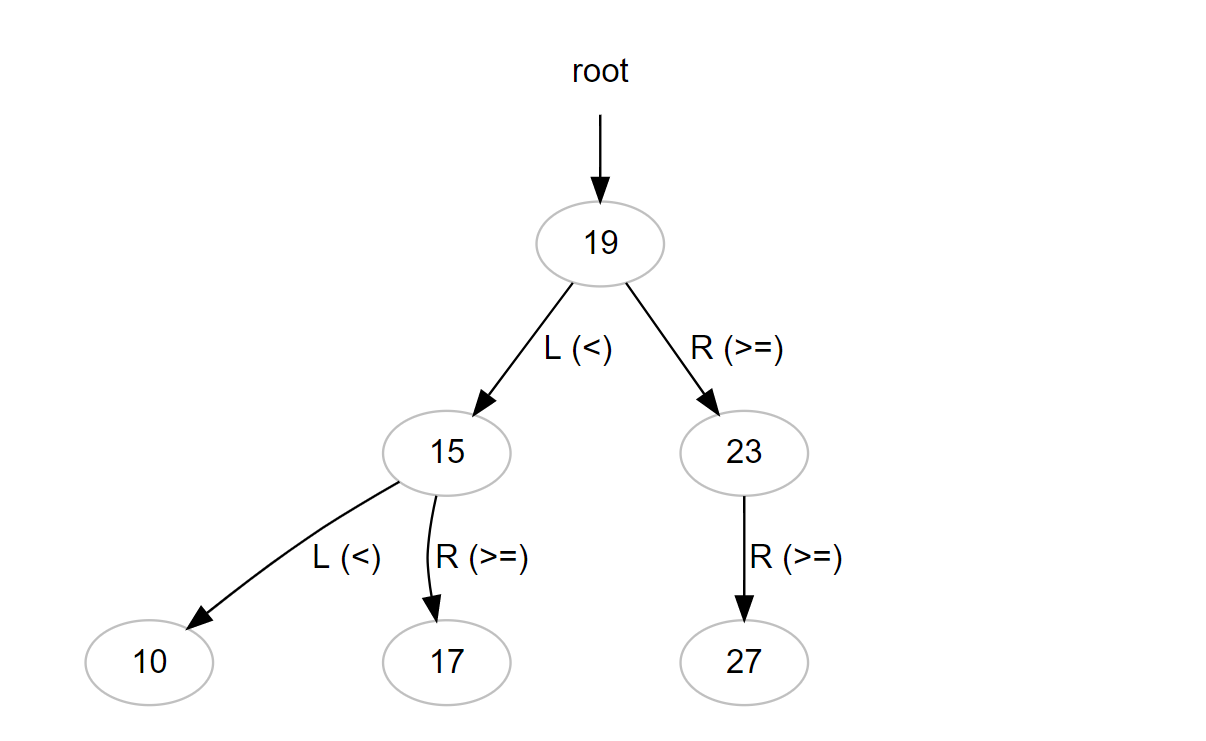
\includegraphics[scale=0.15]{BS}
\end{figure}
\end{frame}
%%%%%%%%%%%%%%%%%%%%%%%%%%%%%%%%%%%%
\begin{frame}
\frametitle{Z čeho se skládá binární strom?}

\begin{itemize}
\item kořen = počáteční uzel stromu
\begin{itemize}
    \item vedou z něj hrany přes vnitřní uzly  až do listů, kde cesta končí.
\end{itemize}

\item vnitřní uzly = nachází se na cestě od listů ke kořeni
\begin{itemize}
\item předchůdci =  jsou blíže kořeni
\item násleníci = jsou dále od kořene
\end{itemize}
\item listy = poslední potomci každé větve stromu
\item rodič = uzel, ze kterého vychází jeho potomci

\item potomci = každý uzel může mít nejvýše dva potomky
\begin{itemize}
\item dělí se pak na:
\begin{itemize}
    \item levý podstrom
    \item pravý podstrom
\end{itemize}
\end{itemize}
\end{itemize}
\end{frame}
%%%%%%%%%%%%%%%%%%%%%%%%%%%%%%%%%%%%
\begin{frame}
\frametitle{Vyhledávací binární strom}
\begin{itemize}
\item uzly obsahují vzájemně porovnatelné klíče
\item levý podstrom 
\begin{itemize}
\item klíče všech uzlů jsou menší, nebo rovny než klíč aktuálního uzlu
\end{itemize}

\item pravý podstrom
\begin{itemize}
\item klíče uzlů jsou větší než klíč aktuálního uzlu
\end{itemize}
\item pokud se neuvažuje vícenásobný výskyt klíčů, pak na obou stranách bude mezi klíči platit ostrá nerovnost
\end{itemize}
\begin{figure}
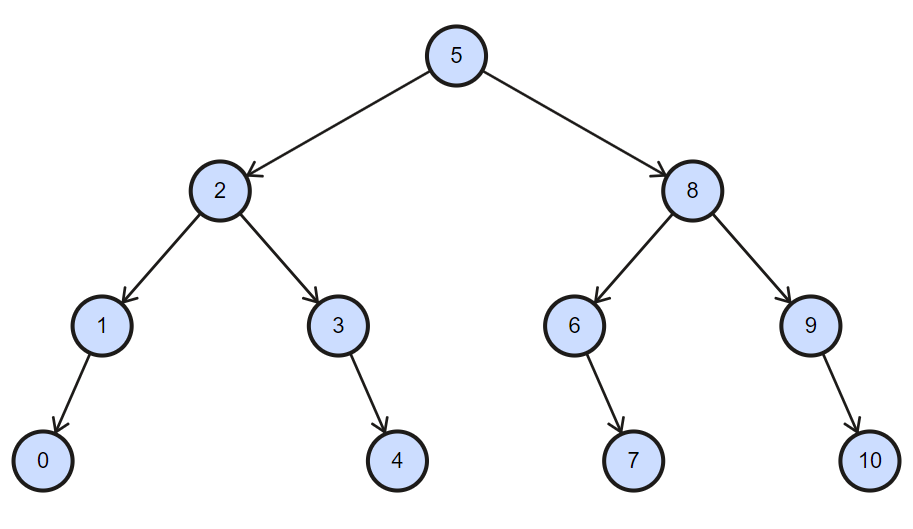
\includegraphics[scale=0.4]{VBS}
\end{figure}
\end{frame}
%%%%%%%%%%%%%%%%%%%%%%%%%%%%%%%%%%%%
\begin{frame}
\frametitle{Příklad funkce insert v binárním vyhledávacím stromu}
\begin{algorithm}[H]
    \SetNlSty{}{}{:}
    \SetNlSkip{-1.15em}
    \Indp\Indpp
    \uIf {$(!root)$}
    {
        root = new Node(key, value);
    }\uElseIf {(key == root\textrightarrow key)}
    {
        root\textrightarrow value = value;
    }\uElseIf {(key $<$ root\textrightarrow key)}
    {
        insert(root\textrightarrow left, key, value);
    }
    \uElse
    {
        insert(root\textrightarrow right, key, value);
    }
    \caption{Void insert(Node*\& root, int key, int value)}
\end{algorithm}
\end{frame}
%%%%%%%%%%%%%%%%%%%%%%%%%%%%%%%%%%%%
\begin{frame}
\frametitle{Popis algoritmu \texttt{insert}}
\begin{itemize}
\item funkce \texttt{insert} začíná hledáním
\item pokud klíč není stejný jako kořen, prohledáme nejdříve levý/pravý podstrom
\item po zjištění hodnoty kořene, vložíme rekurzivně nový uzel do
\begin{itemize}
\item levého podstromu, pokud je jeho klíč menší než hodnota kořene
\item pravého podstromu, pokud je jeho klíč větší nebo roven kořenu
\end{itemize}
\item nakonec se dostaneme k hledanému uzlu a přidáme nový uzel s hodnotu klíče (newNode)

\end{itemize}
\end{frame}
%%%%%%%%%%%%%%%%%%%%%%%%%%%%%%%%%%%%
\begin{frame}{Použité zdroje}
	\begin{itemize}
		\item Binární strom (binary tree)
		 \url{https://cutt.ly/KbvqeRW}

		\item Binární strom
		 \url{https://cutt.ly/FbvqrLe}

		\item Binární vyhledávací strom
		\url{https://cutt.ly/3bvqtXH}
		
	    \item Binary tree \url{https://cutt.ly/SbYg3eu}

	\end{itemize}
\end{frame}
%%%%%%%%%%%%%%%%%%%%%%%%%%%%%%%%%%%%
\end{document}
